% !Mode:: "TeX:UTF-8" 

\BiSection{2.10}{Figures}

\fancyhead[R]{本题2.10由QC.Z完成}

对于图2.52的每个电路,画出$V_X$和$I_X$关于时间的函数曲线草图。$C_1$,$C_2$的初始电压分别为1V,3V。

		\begin{figure}[H] %H为当前位置,!htb为忽略美学标准,htbp为浮动图形
	\begin{minipage}{\linewidth}
		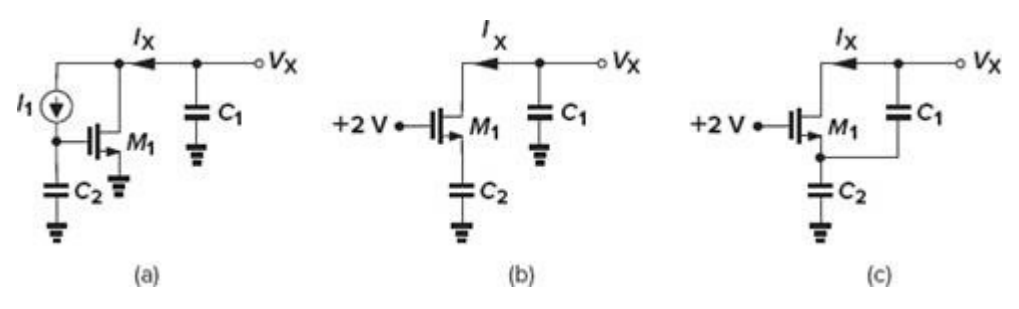
\includegraphics[width=1\linewidth]{2.10.52}
	\end{minipage}
	\caption*{图2.52} %最终文档中希望显示的图片标题
\end{figure}

解:

\scalebox{3}{(a)}

		\begin{figure}[H] %H为当前位置,!htb为忽略美学标准,htbp为浮动图形
	\begin{minipage}{\linewidth}
		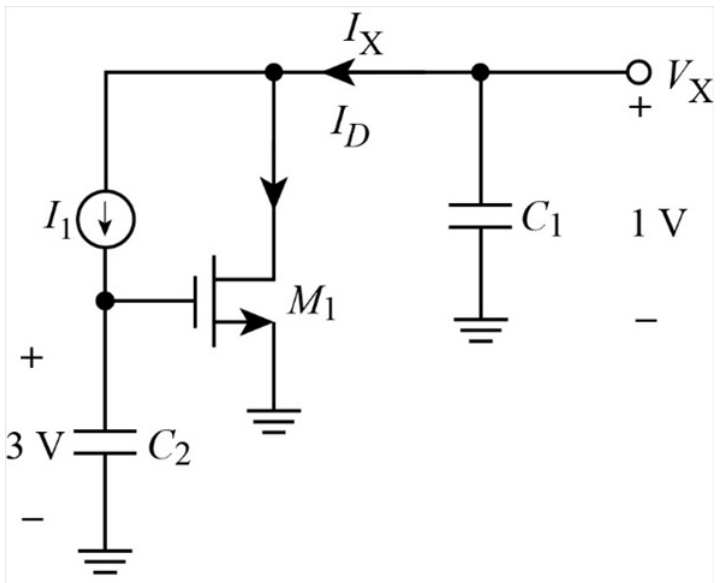
\includegraphics[width=1\linewidth]{2.10-1}
	\end{minipage}
	\caption*{图1} %最终文档中希望显示的图片标题
\end{figure}

$V_G=3V+\frac{I_1}{C_2}t$

当$t=\infty$时,$V_G=\infty$,NFET漏电流为负并且源漏电压等于0。因为$I_X=I_1$后源漏交换并且X点变负。在这条件下,NFET在线性区。

$I_D=\mu_nC_{ox}\frac{W}{L}[(V_{G}-V_{TH})V_{X}-\frac{1}{2}V_{X}^2]=\mu_nC_{ox}\frac{W}{L}\{[3V+\frac{I_1}{C_2}t-0.7V]V_{X}-\frac{1}{2}V_{X}^2\}$

$I_X=I_1+I_D$

$I_X=-C_1\frac{dV_X}{dt}$

		\begin{figure}[H] %H为当前位置,!htb为忽略美学标准,htbp为浮动图形
	\begin{minipage}{\linewidth}
		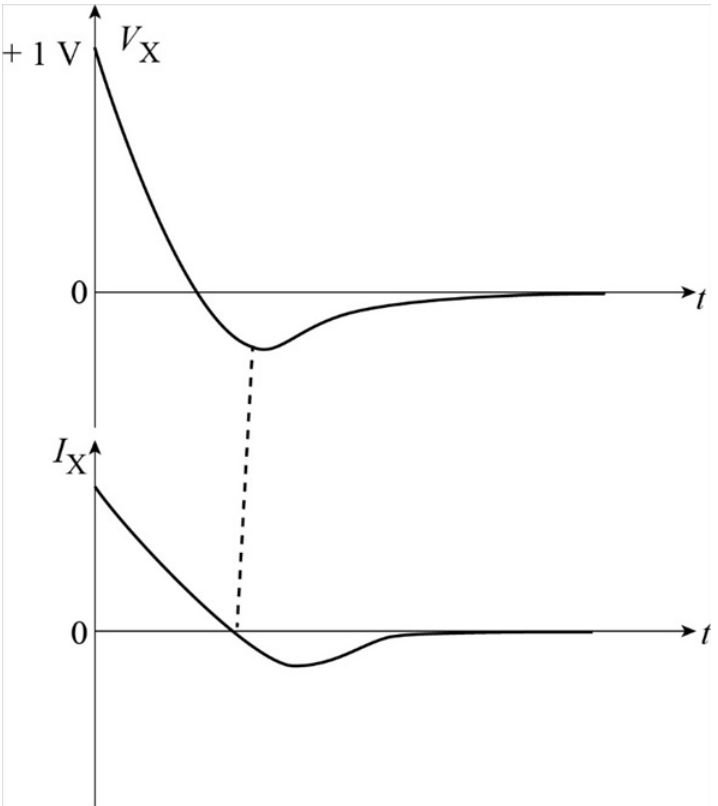
\includegraphics[width=1\linewidth]{2.10-2}
	\end{minipage}
	\caption*{图2} %最终文档中希望显示的图片标题
\end{figure}

\color{blue}{
	
	\{
	
	开始至$V_X$降为0这段时间内,NFET在线性区,电子从$C_1$跑到$C_2$并且经$M_1$跑向地即$I_X=I_1+I_D$;
	
	$V_X$为0时,NFET关,电流源电流全部从$C_1$抽取因此$I_X=I_1 \neq 0$;
	
	由于电流源从$C_1$抽取电流(即把$C_2$电子移动到$C_1$),因此$V_X$变负并且绝对值增大($C_1$得到电子所以电压变负并且电压绝对值增长),$M_1$源漏极交换并且电流反向流动回到线性区,这时电流源电流由$C_1$和$M_1$共同提供$I_1=I_X+I_D$(即$I_X=I_1-I_D$,$I_X$继续减小);
	
	之后$I_X$不断减小直至0即$I_1=I_D$,这时电流源电流完全由$M_1$提供;
	
	由于电流源通过$M_1$从地抽取电流(即把$C_2$电子移动到地),$M_1$的$V_{GS}$增大,根据线性区公式$M_1$电流绝对值增大并且多出来的电流流向$C_1$($C_1$失去电子)即$I_D=I_1+I_X$,因此$V_X$绝对值减小(同时得到结论:之前的临界条件为$V_X$负增长至极值,从电容公式也可以看出来导数为0对应极值);
	
	之后由于$V_X$绝对值减小即$M_1$的$V_{DS}$减小,根据线性区公式$I_D$绝对值先因为$V_{GS}$增大而增大然后因为$V_{DS}$减小而减小,$I_X=I_D-I_1$由于$I_1$不变因此$I_X$趋势相同;
	
	$I_X$更快接近0是因为如果慢则$I_X$大会导致$V_X$迅速接近0(导函数较大则原函数减小较快),并且由于线性区的$M_1$的$V_{GS}$越来越大,$M_1$的$V_{DS}$不需要很大也能保证电流源的电流(合理性)但是为了满足电流源电流($I_D=I_1$)不能减小太快稍微要等$M_1$的$V_{GS}$增大否则$M_1$电流变小无法满足电流源需求。
	
	\}
	
}


\color{black}{
	
}

\scalebox{3}{(b)}

		\begin{figure}[H] %H为当前位置,!htb为忽略美学标准,htbp为浮动图形
	\begin{minipage}{\linewidth}
		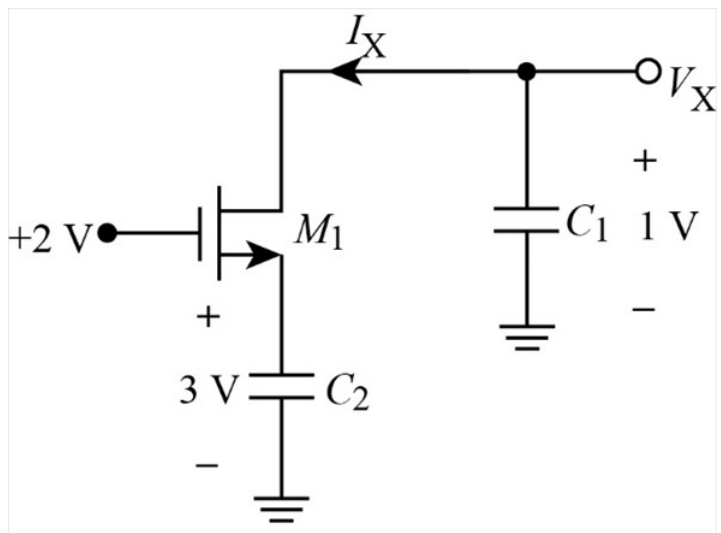
\includegraphics[width=1\linewidth]{2.10-3}
	\end{minipage}
	\caption*{图3} %最终文档中希望显示的图片标题
\end{figure}

NFET源漏交换

\begin{figure}[H] %H为当前位置,!htb为忽略美学标准,htbp为浮动图形
	\begin{minipage}{\linewidth}
		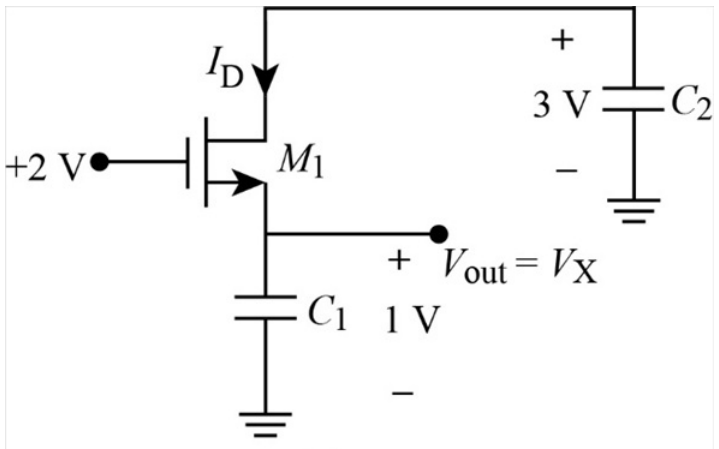
\includegraphics[width=1\linewidth]{2.10-4}
	\end{minipage}
	\caption*{图4} %最终文档中希望显示的图片标题
\end{figure}

$I_D=\frac{dq}{dt}$

$V_X=1V+\frac{q}{C_1}$\ding{172}

$V_D=V_{C2}=3V-\frac{q}{C_2}$\ding{173}

当$V_G-V_X<V_{TH}$即$V_X>1.3V$时,NFET关

当$V_G-V_{TH}<V_D$即$V_D=3V-\frac{q}{C_2}>1.3V$时,NFET在饱和区\textcolor{blue}{(下面计算为满足这个条件,$C_1$与$C_2$的约束)}

$V_X(t)=1V+\frac{q(t)}{C_1}$\ding{172}

$V_X(\infty)=1V+\frac{q(\infty)}{C_1}$

$1.3V=1V+\frac{q(\infty)}{C_1}$

$q(\infty)=(0.3V)C_1$

$V_D(t)=3V-\frac{q(t)}{C_2}$\ding{173}

$V_D(\infty)=3V-\frac{q(\infty)}{C_2}$

$V_D(\infty)=3V-\frac{(0.3V)C_1}{C_2}>1.3V$

$C_1<5.67C_2$

$I_D=\frac{1}{2}\mu_nC_{ox}\frac{W}{L}(2V-1V-\frac{q}{C_1}-0.7V)^2$

$\frac{dq}{dt}=\frac{1}{2}\mu_nC_{ox}\frac{W}{L}(0.3V-\frac{q}{C_1})^2$

$\frac{dq}{(0.3V-\frac{q}{C_1})^2}=(\frac{1}{2}\mu_nC_{ox}\frac{W}{L})dt$

$\frac{\frac{dq}{C_1}}{(0.3V-\frac{q}{C_1})^2}=(\frac{1}{2}\mu_nC_{ox}\frac{W}{L})(\frac{1}{C_1})dt$

令$\alpha=(\frac{1}{2}\mu_nC_{ox}\frac{W}{L})(\frac{1}{C_1})$

$\int \frac{\frac{dq}{C_1}}{(0.3V-\frac{q}{C_1})^2}=\alpha \int dt$

$\alpha t=\frac{1}{0.3V-\frac{q}{C_1}}+k$\ding{174}

$(\alpha) (0)=\frac{1}{0.3V-\frac{(0)}{C_1}}+k$

$k=-\frac{1}{0.3V}$

将上式代入\ding{174}

$\alpha t=\frac{1}{0.3V-\frac{q}{C_1}}-\frac{1}{0.3V}$

$\alpha t+\frac{1}{0.3V}=\frac{1}{0.3V-\frac{q}{C_1}}$

$0.3V-\frac{q}{C_1}=\frac{1}{\alpha t+\frac{1}{0.3V}}$

$\frac{q}{C_1}=0.3V-\frac{1}{\alpha t+\frac{1}{0.3V}}$

将上式代入\ding{172}

$V_X=1V+0.3V-\frac{1}{\alpha t+\frac{1}{0.3V}}$

$I_X=-C_1\frac{dV_X}{dt}$

联立以上二式

$I_X=-C_1\frac{d}{dt}(1.3V-\frac{1}{\alpha t+\frac{1}{0.3V}})=-\frac{\alpha C_1}{(\alpha t+\frac{1}{0.3V})^2}$

\begin{figure}[H] %H为当前位置,!htb为忽略美学标准,htbp为浮动图形
	\begin{minipage}{\linewidth}
		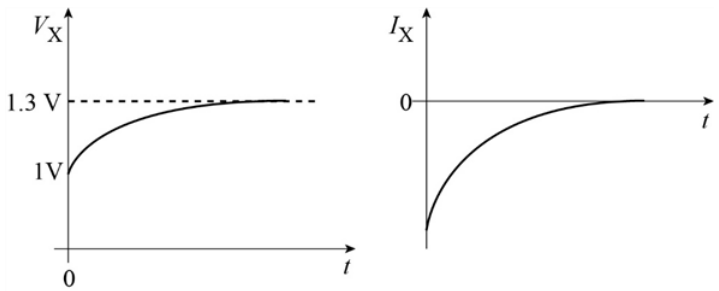
\includegraphics[width=1\linewidth]{2.10-5}
	\end{minipage}
	\caption*{图5} %最终文档中希望显示的图片标题
\end{figure}

\scalebox{3}{(c)}

\begin{figure}[H] %H为当前位置,!htb为忽略美学标准,htbp为浮动图形
	\begin{minipage}{\linewidth}
		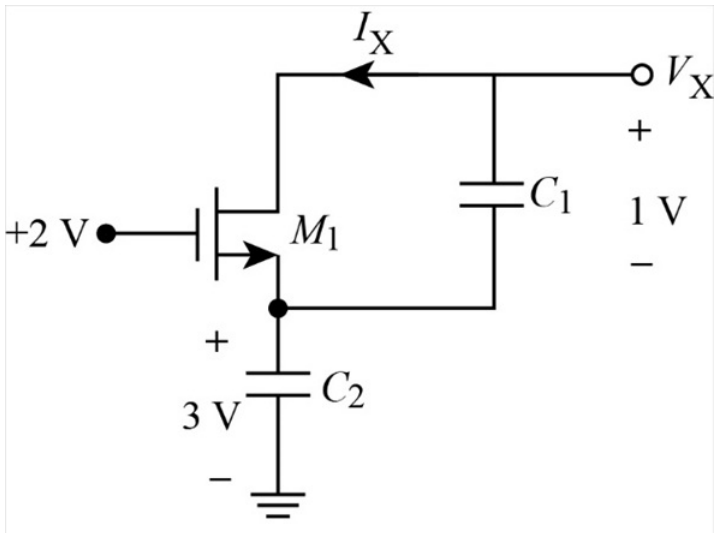
\includegraphics[width=1\linewidth]{2.10-6}
	\end{minipage}
	\caption*{图6} %最终文档中希望显示的图片标题
\end{figure}

$V_G-V_{C2}<V_{TH}$即$-1V<0.7V$,NFET关

\begin{figure}[H] %H为当前位置,!htb为忽略美学标准,htbp为浮动图形
	\begin{minipage}{\linewidth}
		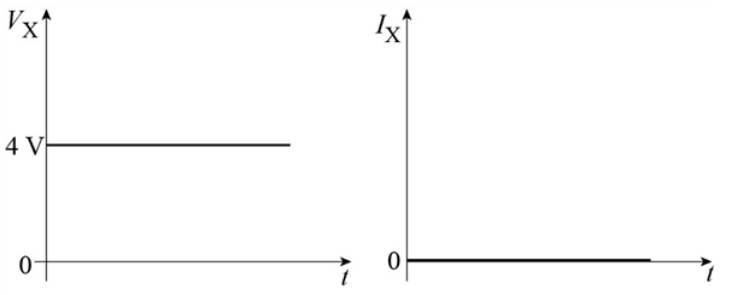
\includegraphics[width=1\linewidth]{2.10-7}
	\end{minipage}
	\caption*{图7} %最终文档中希望显示的图片标题
\end{figure}












